\documentclass[twoside]{book}

% Packages required by doxygen
\usepackage{fixltx2e}
\usepackage{calc}
\usepackage{doxygen}
\usepackage[export]{adjustbox} % also loads graphicx
\usepackage{graphicx}
\usepackage[utf8]{inputenc}
\usepackage{makeidx}
\usepackage{multicol}
\usepackage{multirow}
\PassOptionsToPackage{warn}{textcomp}
\usepackage{textcomp}
\usepackage[nointegrals]{wasysym}
\usepackage[table]{xcolor}

% Font selection
\usepackage[T1]{fontenc}
\usepackage[scaled=.90]{helvet}
\usepackage{courier}
\usepackage{amssymb}
\usepackage{sectsty}
\renewcommand{\familydefault}{\sfdefault}
\allsectionsfont{%
  \fontseries{bc}\selectfont%
  \color{darkgray}%
}
\renewcommand{\DoxyLabelFont}{%
  \fontseries{bc}\selectfont%
  \color{darkgray}%
}
\newcommand{\+}{\discretionary{\mbox{\scriptsize$\hookleftarrow$}}{}{}}

% Page & text layout
\usepackage{geometry}
\geometry{%
  a4paper,%
  top=2.5cm,%
  bottom=2.5cm,%
  left=2.5cm,%
  right=2.5cm%
}
\tolerance=750
\hfuzz=15pt
\hbadness=750
\setlength{\emergencystretch}{15pt}
\setlength{\parindent}{0cm}
\setlength{\parskip}{0.2cm}
\makeatletter
\renewcommand{\paragraph}{%
  \@startsection{paragraph}{4}{0ex}{-1.0ex}{1.0ex}{%
    \normalfont\normalsize\bfseries\SS@parafont%
  }%
}
\renewcommand{\subparagraph}{%
  \@startsection{subparagraph}{5}{0ex}{-1.0ex}{1.0ex}{%
    \normalfont\normalsize\bfseries\SS@subparafont%
  }%
}
\makeatother

% Headers & footers
\usepackage{fancyhdr}
\pagestyle{fancyplain}
\fancyhead[LE]{\fancyplain{}{\bfseries\thepage}}
\fancyhead[CE]{\fancyplain{}{}}
\fancyhead[RE]{\fancyplain{}{\bfseries\leftmark}}
\fancyhead[LO]{\fancyplain{}{\bfseries\rightmark}}
\fancyhead[CO]{\fancyplain{}{}}
\fancyhead[RO]{\fancyplain{}{\bfseries\thepage}}
\fancyfoot[LE]{\fancyplain{}{}}
\fancyfoot[CE]{\fancyplain{}{}}
\fancyfoot[RE]{\fancyplain{}{\bfseries\scriptsize Generated on Thu Dec 10 2015 20\+:36\+:08 for Project2\+Minesweeper by Doxygen }}
\fancyfoot[LO]{\fancyplain{}{\bfseries\scriptsize Generated on Thu Dec 10 2015 20\+:36\+:08 for Project2\+Minesweeper by Doxygen }}
\fancyfoot[CO]{\fancyplain{}{}}
\fancyfoot[RO]{\fancyplain{}{}}
\renewcommand{\footrulewidth}{0.4pt}
\renewcommand{\chaptermark}[1]{%
  \markboth{#1}{}%
}
\renewcommand{\sectionmark}[1]{%
  \markright{\thesection\ #1}%
}

% Indices & bibliography
\usepackage{natbib}
\usepackage[titles]{tocloft}
\setcounter{tocdepth}{3}
\setcounter{secnumdepth}{5}
\makeindex

% Hyperlinks (required, but should be loaded last)
\usepackage{ifpdf}
\ifpdf
  \usepackage[pdftex,pagebackref=true]{hyperref}
\else
  \usepackage[ps2pdf,pagebackref=true]{hyperref}
\fi
\hypersetup{%
  colorlinks=true,%
  linkcolor=blue,%
  citecolor=blue,%
  unicode%
}

% Custom commands
\newcommand{\clearemptydoublepage}{%
  \newpage{\pagestyle{empty}\cleardoublepage}%
}


%===== C O N T E N T S =====

\begin{document}

% Titlepage & ToC
\hypersetup{pageanchor=false,
             bookmarks=true,
             bookmarksnumbered=true,
             pdfencoding=unicode
            }
\pagenumbering{roman}
\begin{titlepage}
\vspace*{7cm}
\begin{center}%
{\Large Project2\+Minesweeper }\\
\vspace*{1cm}
{\large Generated by Doxygen 1.8.10}\\
\vspace*{0.5cm}
{\small Thu Dec 10 2015 20:36:08}\\
\end{center}
\end{titlepage}
\clearemptydoublepage
\tableofcontents
\clearemptydoublepage
\pagenumbering{arabic}
\hypersetup{pageanchor=true}

%--- Begin generated contents ---
\chapter{Hierarchical Index}
\section{Class Hierarchy}
This inheritance list is sorted roughly, but not completely, alphabetically\+:\begin{DoxyCompactList}
\item \contentsline{section}{Abstracts}{\pageref{class_abstracts}}{}
\begin{DoxyCompactList}
\item \contentsline{section}{Game\+Board}{\pageref{class_game_board}}{}
\begin{DoxyCompactList}
\item \contentsline{section}{Minesweeper}{\pageref{class_minesweeper}}{}
\end{DoxyCompactList}
\end{DoxyCompactList}
\item \contentsline{section}{Game$<$ T $>$}{\pageref{class_game}}{}
\item \contentsline{section}{Game\+Board\+:\+:wrong}{\pageref{class_game_board_1_1wrong}}{}
\end{DoxyCompactList}

\chapter{Class Index}
\section{Class List}
Here are the classes, structs, unions and interfaces with brief descriptions\+:\begin{DoxyCompactList}
\item\contentsline{section}{\hyperlink{class_abstracts}{Abstracts} }{\pageref{class_abstracts}}{}
\item\contentsline{section}{\hyperlink{class_game}{Game$<$ T $>$} }{\pageref{class_game}}{}
\item\contentsline{section}{\hyperlink{class_game_board}{Game\+Board} \\*Base class for games that require an n$\ast$m array such as minesweeper }{\pageref{class_game_board}}{}
\item\contentsline{section}{\hyperlink{class_minesweeper}{Minesweeper} }{\pageref{class_minesweeper}}{}
\item\contentsline{section}{\hyperlink{class_game_board_1_1wrong}{Game\+Board\+::wrong} \\*Output this if user tries to set negative rows or columns }{\pageref{class_game_board_1_1wrong}}{}
\end{DoxyCompactList}

\chapter{File Index}
\section{File List}
Here is a list of all files with brief descriptions\+:\begin{DoxyCompactList}
\item\contentsline{section}{\hyperlink{_8dep_8inc}{.\+dep.\+inc} }{\pageref{_8dep_8inc}}{}
\item\contentsline{section}{\hyperlink{_abstracts_8h}{Abstracts.\+h} }{\pageref{_abstracts_8h}}{}
\item\contentsline{section}{\hyperlink{_game_board_8cpp}{Game\+Board.\+cpp} }{\pageref{_game_board_8cpp}}{}
\item\contentsline{section}{\hyperlink{_game_board_8h}{Game\+Board.\+h} }{\pageref{_game_board_8h}}{}
\item\contentsline{section}{\hyperlink{main_8cpp}{main.\+cpp} }{\pageref{main_8cpp}}{}
\item\contentsline{section}{\hyperlink{_minesweeper_8cpp}{Minesweeper.\+cpp} }{\pageref{_minesweeper_8cpp}}{}
\item\contentsline{section}{\hyperlink{_minesweeper_8h}{Minesweeper.\+h} }{\pageref{_minesweeper_8h}}{}
\item\contentsline{section}{\hyperlink{_templates_8h}{Templates.\+h} }{\pageref{_templates_8h}}{}
\end{DoxyCompactList}

\chapter{Class Documentation}
\hypertarget{class_abstracts}{}\section{Abstracts Class Reference}
\label{class_abstracts}\index{Abstracts@{Abstracts}}


{\ttfamily \#include $<$Abstracts.\+h$>$}

Inheritance diagram for Abstracts\+:\begin{figure}[H]
\begin{center}
\leavevmode
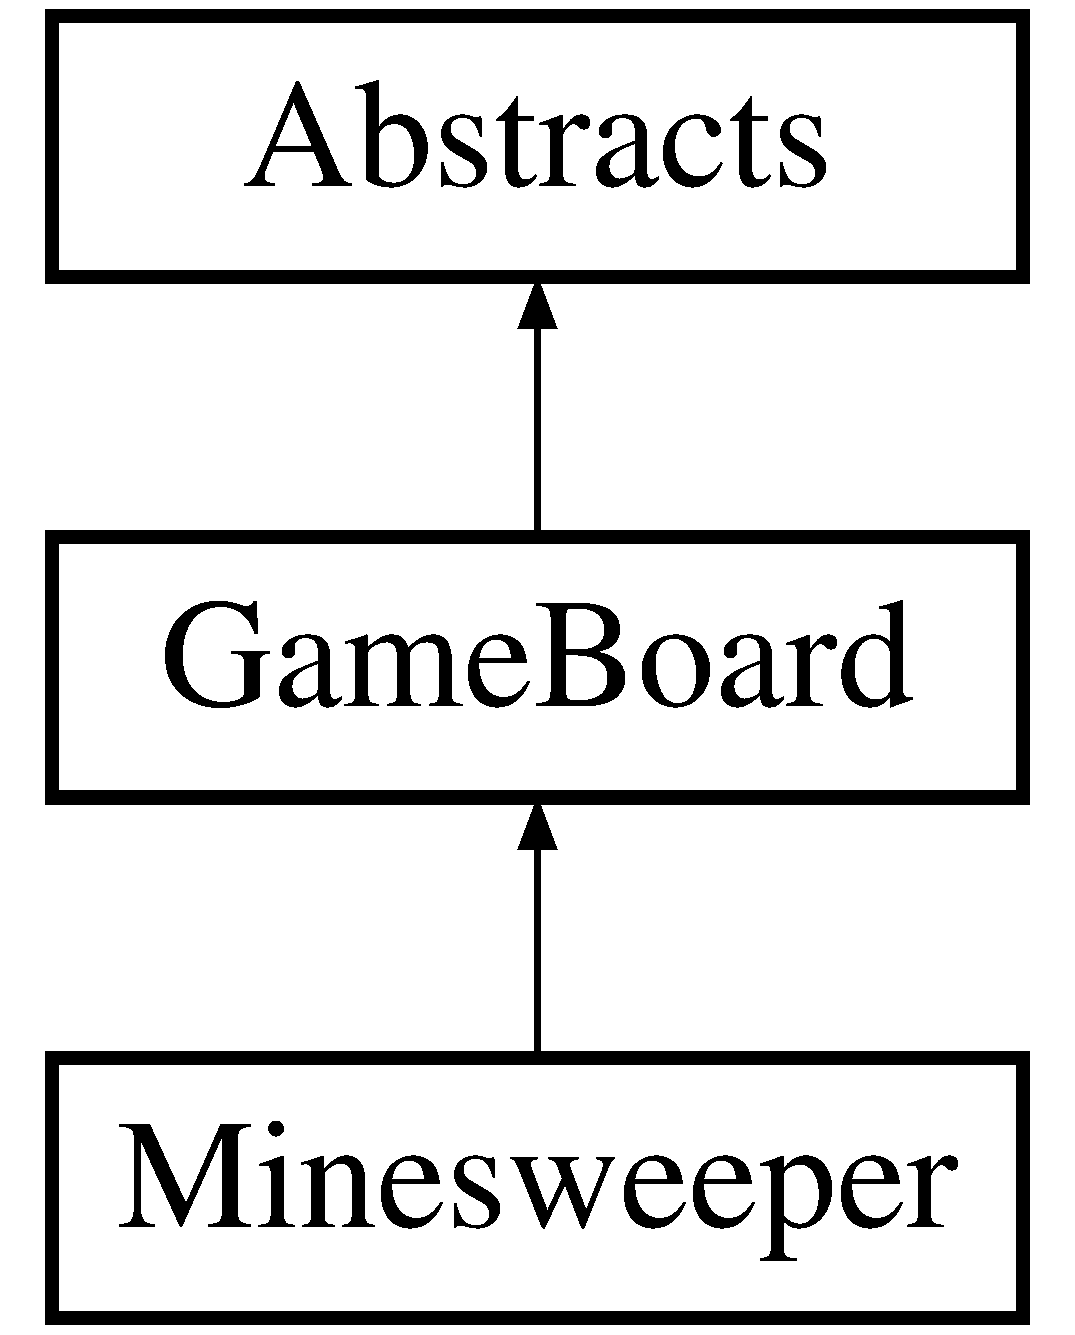
\includegraphics[height=3.000000cm]{class_abstracts}
\end{center}
\end{figure}
\subsection*{Protected Member Functions}
\begin{DoxyCompactItemize}
\item 
virtual void \hyperlink{class_abstracts_af4eaab1bfc282612adfaca1eb2461b66}{set\+Rows} (int)=0
\item 
virtual void \hyperlink{class_abstracts_aa8bda3c5e2165c34ad51b1833cb5ce58}{set\+Cols} (int)=0
\item 
virtual int \hyperlink{class_abstracts_adb4bf4c040da9691558d27991db6c33f}{get\+Rows} () const  =0
\item 
virtual int \hyperlink{class_abstracts_a34a6f65f6f9dea6a2e6014b76b333b6a}{get\+Cols} () const  =0
\item 
virtual void \hyperlink{class_abstracts_ad8fa8c3873a0c5b593887ae924fe6fce}{set\+Up\+G} ()=0
\item 
virtual void \hyperlink{class_abstracts_a2355084469196dff6645993ff14c96bd}{print} () const  =0
\end{DoxyCompactItemize}


\subsection{Member Function Documentation}
\hypertarget{class_abstracts_a34a6f65f6f9dea6a2e6014b76b333b6a}{}\index{Abstracts@{Abstracts}!get\+Cols@{get\+Cols}}
\index{get\+Cols@{get\+Cols}!Abstracts@{Abstracts}}
\subsubsection[{get\+Cols() const  =0}]{\setlength{\rightskip}{0pt plus 5cm}virtual int Abstracts\+::get\+Cols (
\begin{DoxyParamCaption}
{}
\end{DoxyParamCaption}
) const\hspace{0.3cm}{\ttfamily [protected]}, {\ttfamily [pure virtual]}}\label{class_abstracts_a34a6f65f6f9dea6a2e6014b76b333b6a}


Implemented in \hyperlink{class_minesweeper_a82c571f6a7a80d001a3cb0a73445588f}{Minesweeper}, and \hyperlink{class_game_board_a3e72c802e556c00efd911d95986a4f2e}{Game\+Board}.

\hypertarget{class_abstracts_adb4bf4c040da9691558d27991db6c33f}{}\index{Abstracts@{Abstracts}!get\+Rows@{get\+Rows}}
\index{get\+Rows@{get\+Rows}!Abstracts@{Abstracts}}
\subsubsection[{get\+Rows() const  =0}]{\setlength{\rightskip}{0pt plus 5cm}virtual int Abstracts\+::get\+Rows (
\begin{DoxyParamCaption}
{}
\end{DoxyParamCaption}
) const\hspace{0.3cm}{\ttfamily [protected]}, {\ttfamily [pure virtual]}}\label{class_abstracts_adb4bf4c040da9691558d27991db6c33f}


Implemented in \hyperlink{class_minesweeper_abf6ccbfbecf96ef15f21ca7a94e98f1b}{Minesweeper}, and \hyperlink{class_game_board_a06b193fdd5b618efdbb2700fd7dcffd0}{Game\+Board}.

\hypertarget{class_abstracts_a2355084469196dff6645993ff14c96bd}{}\index{Abstracts@{Abstracts}!print@{print}}
\index{print@{print}!Abstracts@{Abstracts}}
\subsubsection[{print() const  =0}]{\setlength{\rightskip}{0pt plus 5cm}virtual void Abstracts\+::print (
\begin{DoxyParamCaption}
{}
\end{DoxyParamCaption}
) const\hspace{0.3cm}{\ttfamily [protected]}, {\ttfamily [pure virtual]}}\label{class_abstracts_a2355084469196dff6645993ff14c96bd}


Implemented in \hyperlink{class_minesweeper_ac158ba4f4bca146302059096db943dad}{Minesweeper}, and \hyperlink{class_game_board_a90f93cc1b6ca4e06f7200696fb21c9b9}{Game\+Board}.

\hypertarget{class_abstracts_aa8bda3c5e2165c34ad51b1833cb5ce58}{}\index{Abstracts@{Abstracts}!set\+Cols@{set\+Cols}}
\index{set\+Cols@{set\+Cols}!Abstracts@{Abstracts}}
\subsubsection[{set\+Cols(int)=0}]{\setlength{\rightskip}{0pt plus 5cm}virtual void Abstracts\+::set\+Cols (
\begin{DoxyParamCaption}
\item[{int}]{}
\end{DoxyParamCaption}
)\hspace{0.3cm}{\ttfamily [protected]}, {\ttfamily [pure virtual]}}\label{class_abstracts_aa8bda3c5e2165c34ad51b1833cb5ce58}


Implemented in \hyperlink{class_minesweeper_a6e243fa0d9859fcf6dc4e45ec146b7df}{Minesweeper}, and \hyperlink{class_game_board_a84673c141f4790940df3aca0e24c3203}{Game\+Board}.

\hypertarget{class_abstracts_af4eaab1bfc282612adfaca1eb2461b66}{}\index{Abstracts@{Abstracts}!set\+Rows@{set\+Rows}}
\index{set\+Rows@{set\+Rows}!Abstracts@{Abstracts}}
\subsubsection[{set\+Rows(int)=0}]{\setlength{\rightskip}{0pt plus 5cm}virtual void Abstracts\+::set\+Rows (
\begin{DoxyParamCaption}
\item[{int}]{}
\end{DoxyParamCaption}
)\hspace{0.3cm}{\ttfamily [protected]}, {\ttfamily [pure virtual]}}\label{class_abstracts_af4eaab1bfc282612adfaca1eb2461b66}


Implemented in \hyperlink{class_minesweeper_ab316cfe272f38e4768a6e45c171bce3a}{Minesweeper}, and \hyperlink{class_game_board_ac8b28f17c3ea049f3cb07216b850c4a9}{Game\+Board}.

\hypertarget{class_abstracts_ad8fa8c3873a0c5b593887ae924fe6fce}{}\index{Abstracts@{Abstracts}!set\+Up\+G@{set\+Up\+G}}
\index{set\+Up\+G@{set\+Up\+G}!Abstracts@{Abstracts}}
\subsubsection[{set\+Up\+G()=0}]{\setlength{\rightskip}{0pt plus 5cm}virtual void Abstracts\+::set\+Up\+G (
\begin{DoxyParamCaption}
{}
\end{DoxyParamCaption}
)\hspace{0.3cm}{\ttfamily [protected]}, {\ttfamily [pure virtual]}}\label{class_abstracts_ad8fa8c3873a0c5b593887ae924fe6fce}


Implemented in \hyperlink{class_minesweeper_ac5ae43be99a0cc126da239d3572acbe7}{Minesweeper}, and \hyperlink{class_game_board_a81f25c1109558131e0153a4b278cffcb}{Game\+Board}.



The documentation for this class was generated from the following file\+:\begin{DoxyCompactItemize}
\item 
\hyperlink{_abstracts_8h}{Abstracts.\+h}\end{DoxyCompactItemize}

\hypertarget{class_game}{}\section{Game$<$ T $>$ Class Template Reference}
\label{class_game}\index{Game$<$ T $>$@{Game$<$ T $>$}}


{\ttfamily \#include $<$Templates.\+h$>$}

\subsection*{Public Member Functions}
\begin{DoxyCompactItemize}
\item 
\hyperlink{class_game_ad75fd91feb6a0dcda2e91f53a79bb882}{Game} ()
\item 
\hyperlink{class_game_ae1e0764e1cc2bbb6b356625de6a6b574}{Game} (T $\ast$t)
\item 
\hyperlink{class_game_ac98b054acf64c7ac2c7c780e79b4f618}{$\sim$\+Game} ()
\item 
\hyperlink{class_game}{Game}$<$ T $>$ \& \hyperlink{class_game_a6f83d7d8fbbd23753ec3251a38aab847}{operator=} (const T \&)
\item 
\hyperlink{class_game_a491b5e73b82732c90942e706a33580e4}{operator bool} ()
\item 
T $\ast$ \hyperlink{class_game_adad3578d9dad72b1989fbce7787e0659}{operator-\/$>$} () const 
\item 
T \& \hyperlink{class_game_a6e4402ebcfeb0a0b0bf8cc9441753001}{operator$\ast$} () const 
\end{DoxyCompactItemize}


\subsection{Constructor \& Destructor Documentation}
\hypertarget{class_game_ad75fd91feb6a0dcda2e91f53a79bb882}{}\index{Game@{Game}!Game@{Game}}
\index{Game@{Game}!Game@{Game}}
\subsubsection[{Game()}]{\setlength{\rightskip}{0pt plus 5cm}template$<$class T$>$ {\bf Game}$<$ T $>$\+::{\bf Game} (
\begin{DoxyParamCaption}
{}
\end{DoxyParamCaption}
)\hspace{0.3cm}{\ttfamily [inline]}}\label{class_game_ad75fd91feb6a0dcda2e91f53a79bb882}
\hypertarget{class_game_ae1e0764e1cc2bbb6b356625de6a6b574}{}\index{Game@{Game}!Game@{Game}}
\index{Game@{Game}!Game@{Game}}
\subsubsection[{Game(\+T $\ast$t)}]{\setlength{\rightskip}{0pt plus 5cm}template$<$class T$>$ {\bf Game}$<$ T $>$\+::{\bf Game} (
\begin{DoxyParamCaption}
\item[{T $\ast$}]{t}
\end{DoxyParamCaption}
)\hspace{0.3cm}{\ttfamily [inline]}}\label{class_game_ae1e0764e1cc2bbb6b356625de6a6b574}
\hypertarget{class_game_ac98b054acf64c7ac2c7c780e79b4f618}{}\index{Game@{Game}!````~Game@{$\sim$\+Game}}
\index{````~Game@{$\sim$\+Game}!Game@{Game}}
\subsubsection[{$\sim$\+Game()}]{\setlength{\rightskip}{0pt plus 5cm}template$<$class T$>$ {\bf Game}$<$ T $>$\+::$\sim${\bf Game} (
\begin{DoxyParamCaption}
{}
\end{DoxyParamCaption}
)\hspace{0.3cm}{\ttfamily [inline]}}\label{class_game_ac98b054acf64c7ac2c7c780e79b4f618}


\subsection{Member Function Documentation}
\hypertarget{class_game_a491b5e73b82732c90942e706a33580e4}{}\index{Game@{Game}!operator bool@{operator bool}}
\index{operator bool@{operator bool}!Game@{Game}}
\subsubsection[{operator bool()}]{\setlength{\rightskip}{0pt plus 5cm}template$<$class T$>$ {\bf Game}$<$ T $>$\+::operator bool (
\begin{DoxyParamCaption}
{}
\end{DoxyParamCaption}
)\hspace{0.3cm}{\ttfamily [inline]}}\label{class_game_a491b5e73b82732c90942e706a33580e4}
\hypertarget{class_game_a6e4402ebcfeb0a0b0bf8cc9441753001}{}\index{Game@{Game}!operator$\ast$@{operator$\ast$}}
\index{operator$\ast$@{operator$\ast$}!Game@{Game}}
\subsubsection[{operator$\ast$() const }]{\setlength{\rightskip}{0pt plus 5cm}template$<$class T $>$ T \& {\bf Game}$<$ T $>$\+::operator$\ast$ (
\begin{DoxyParamCaption}
{}
\end{DoxyParamCaption}
) const}\label{class_game_a6e4402ebcfeb0a0b0bf8cc9441753001}
\hypertarget{class_game_adad3578d9dad72b1989fbce7787e0659}{}\index{Game@{Game}!operator-\/$>$@{operator-\/$>$}}
\index{operator-\/$>$@{operator-\/$>$}!Game@{Game}}
\subsubsection[{operator-\/$>$() const }]{\setlength{\rightskip}{0pt plus 5cm}template$<$class T $>$ T $\ast$ {\bf Game}$<$ T $>$\+::operator-\/$>$ (
\begin{DoxyParamCaption}
{}
\end{DoxyParamCaption}
) const}\label{class_game_adad3578d9dad72b1989fbce7787e0659}
only return p if it points to something \hypertarget{class_game_a6f83d7d8fbbd23753ec3251a38aab847}{}\index{Game@{Game}!operator=@{operator=}}
\index{operator=@{operator=}!Game@{Game}}
\subsubsection[{operator=(const T \&)}]{\setlength{\rightskip}{0pt plus 5cm}template$<$class T $>$ {\bf Game}$<$ T $>$ \& {\bf Game}$<$ T $>$\+::operator= (
\begin{DoxyParamCaption}
\item[{const T \&}]{rhs}
\end{DoxyParamCaption}
)}\label{class_game_a6f83d7d8fbbd23753ec3251a38aab847}


The documentation for this class was generated from the following file\+:\begin{DoxyCompactItemize}
\item 
\hyperlink{_templates_8h}{Templates.\+h}\end{DoxyCompactItemize}

\hypertarget{class_game_board}{}\section{Game\+Board Class Reference}
\label{class_game_board}\index{Game\+Board@{Game\+Board}}


Base class for games that require an n$\ast$m array such as minesweeper.  




{\ttfamily \#include $<$Game\+Board.\+h$>$}

Inheritance diagram for Game\+Board\+:\begin{figure}[H]
\begin{center}
\leavevmode
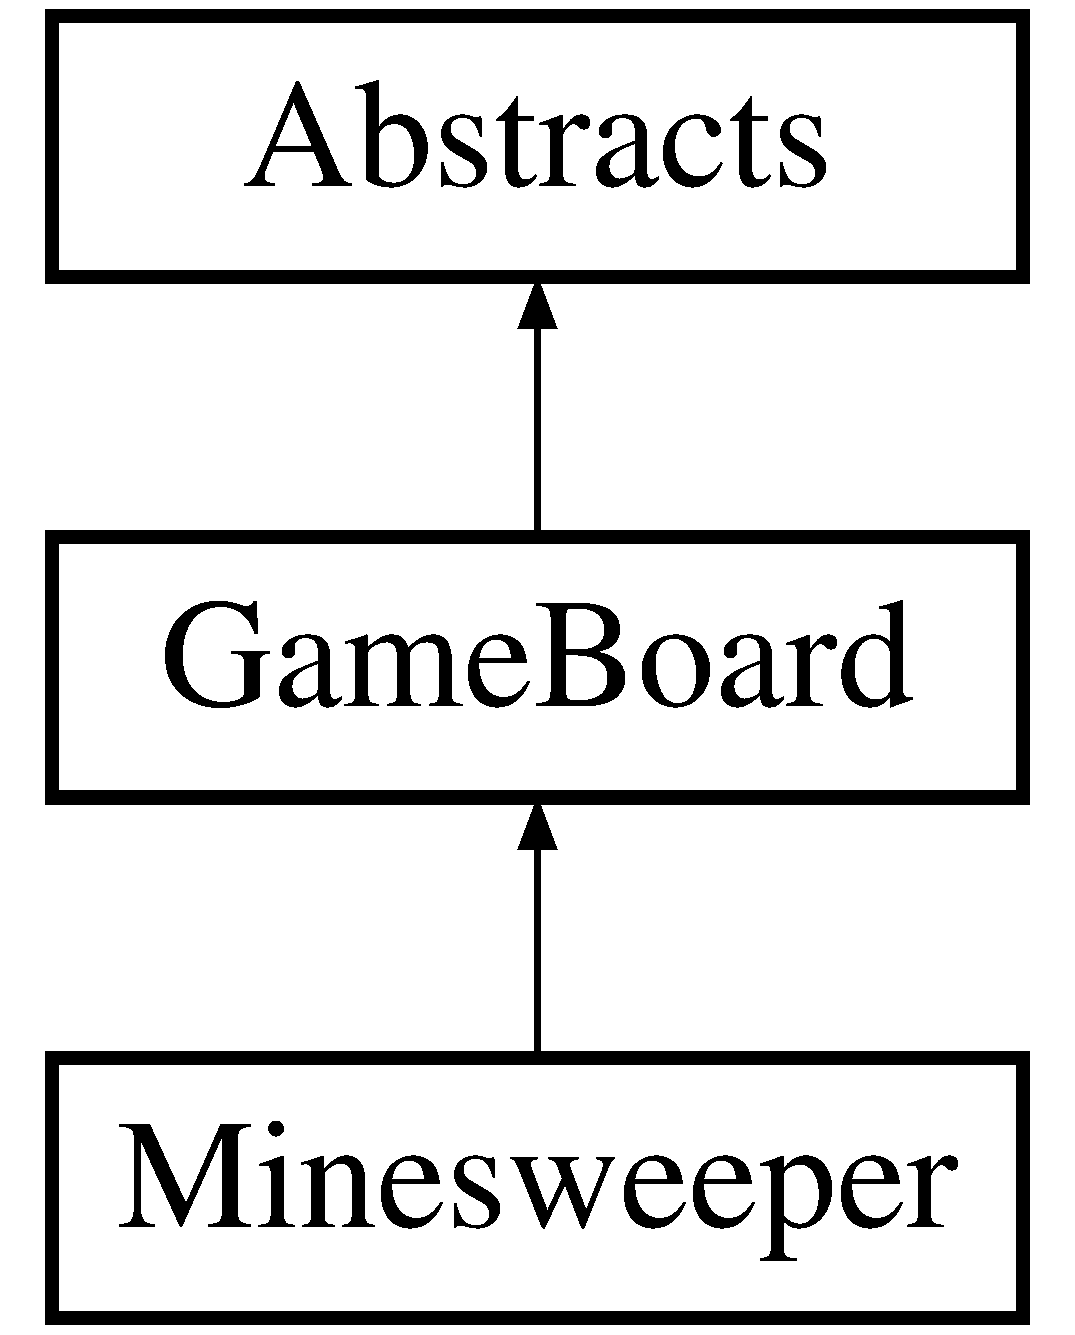
\includegraphics[height=3.000000cm]{class_game_board}
\end{center}
\end{figure}
\subsection*{Classes}
\begin{DoxyCompactItemize}
\item 
class \hyperlink{class_game_board_1_1wrong}{wrong}
\begin{DoxyCompactList}\small\item\em output this if user tries to set negative rows or columns \end{DoxyCompactList}\end{DoxyCompactItemize}
\subsection*{Public Member Functions}
\begin{DoxyCompactItemize}
\item 
\hyperlink{class_game_board_ac9ffda4dde51341af1315168e8e066a0}{Game\+Board} (int \hyperlink{class_game_board_a83b7f30682f1312a911e036b70c1c6d6}{rows}, int \hyperlink{class_game_board_a95d7d4a10285e01d7a12e94e48090cb7}{cols})
\item 
virtual \hyperlink{class_game_board_ae582b50974ecef2810c63516c104ef83}{$\sim$\+Game\+Board} ()
\item 
virtual void \hyperlink{class_game_board_a891a6e8e8983e6ef4f1a19205392d3ef}{destroy} ()
\begin{DoxyCompactList}\small\item\em Function deallocates memory. \end{DoxyCompactList}\item 
virtual void \hyperlink{class_game_board_ac8b28f17c3ea049f3cb07216b850c4a9}{set\+Rows} (int)
\item 
virtual void \hyperlink{class_game_board_a84673c141f4790940df3aca0e24c3203}{set\+Cols} (int)
\item 
virtual int \hyperlink{class_game_board_a06b193fdd5b618efdbb2700fd7dcffd0}{get\+Rows} () const 
\item 
virtual int \hyperlink{class_game_board_a3e72c802e556c00efd911d95986a4f2e}{get\+Cols} () const 
\item 
virtual void \hyperlink{class_game_board_a85f26da7e1be97961225f8fd893f18ee}{clear} ()
\begin{DoxyCompactList}\small\item\em Function resets the \hyperlink{class_game_board}{Game\+Board} to initial in order to use it again. \end{DoxyCompactList}\item 
virtual void \hyperlink{class_game_board_a81f25c1109558131e0153a4b278cffcb}{set\+Up\+G} ()
\item 
virtual void \hyperlink{class_game_board_ac73c2de2d5a31c591ff3434d8fd38686}{load\+Game} ()
\item 
virtual void \hyperlink{class_game_board_a90f93cc1b6ca4e06f7200696fb21c9b9}{print} () const 
\item 
int $\ast$ \hyperlink{class_game_board_a28a159916f1fb80195bc90f065d040fe}{operator\mbox{[}$\,$\mbox{]}} (int index)
\item 
int $\ast$ \hyperlink{class_game_board_acaedf10ba0c53fc745238d528fe8878b}{operator\mbox{[}$\,$\mbox{]}} (int index) const 
\end{DoxyCompactItemize}
\subsection*{Protected Member Functions}
\begin{DoxyCompactItemize}
\item 
virtual void \hyperlink{class_game_board_ab823080e4192fb2673763aa6dea046cd}{create} (int, int)
\begin{DoxyCompactList}\small\item\em Function that creates the grid on which game will be played. \end{DoxyCompactList}\end{DoxyCompactItemize}
\subsection*{Protected Attributes}
\begin{DoxyCompactItemize}
\item 
int $\ast$$\ast$ \hyperlink{class_game_board_aa46b9d2eb5d9baf09f2a6e2a4a777d35}{data}
\item 
int \hyperlink{class_game_board_a83b7f30682f1312a911e036b70c1c6d6}{rows}
\item 
int \hyperlink{class_game_board_a95d7d4a10285e01d7a12e94e48090cb7}{cols}
\end{DoxyCompactItemize}


\subsection{Detailed Description}
Base class for games that require an n$\ast$m array such as minesweeper. 

\subsection{Constructor \& Destructor Documentation}
\hypertarget{class_game_board_ac9ffda4dde51341af1315168e8e066a0}{}\index{Game\+Board@{Game\+Board}!Game\+Board@{Game\+Board}}
\index{Game\+Board@{Game\+Board}!Game\+Board@{Game\+Board}}
\subsubsection[{Game\+Board(int rows, int cols)}]{\setlength{\rightskip}{0pt plus 5cm}Game\+Board\+::\+Game\+Board (
\begin{DoxyParamCaption}
\item[{int}]{rows, }
\item[{int}]{cols}
\end{DoxyParamCaption}
)\hspace{0.3cm}{\ttfamily [inline]}}\label{class_game_board_ac9ffda4dde51341af1315168e8e066a0}
\hypertarget{class_game_board_ae582b50974ecef2810c63516c104ef83}{}\index{Game\+Board@{Game\+Board}!````~Game\+Board@{$\sim$\+Game\+Board}}
\index{````~Game\+Board@{$\sim$\+Game\+Board}!Game\+Board@{Game\+Board}}
\subsubsection[{$\sim$\+Game\+Board()}]{\setlength{\rightskip}{0pt plus 5cm}virtual Game\+Board\+::$\sim$\+Game\+Board (
\begin{DoxyParamCaption}
{}
\end{DoxyParamCaption}
)\hspace{0.3cm}{\ttfamily [inline]}, {\ttfamily [virtual]}}\label{class_game_board_ae582b50974ecef2810c63516c104ef83}


\subsection{Member Function Documentation}
\hypertarget{class_game_board_a85f26da7e1be97961225f8fd893f18ee}{}\index{Game\+Board@{Game\+Board}!clear@{clear}}
\index{clear@{clear}!Game\+Board@{Game\+Board}}
\subsubsection[{clear()}]{\setlength{\rightskip}{0pt plus 5cm}void Game\+Board\+::clear (
\begin{DoxyParamCaption}
{}
\end{DoxyParamCaption}
)\hspace{0.3cm}{\ttfamily [virtual]}}\label{class_game_board_a85f26da7e1be97961225f8fd893f18ee}


Function resets the \hyperlink{class_game_board}{Game\+Board} to initial in order to use it again. 



Reimplemented in \hyperlink{class_minesweeper_a9304b49877a6d02f6e5b9c5f48f34055}{Minesweeper}.

\hypertarget{class_game_board_ab823080e4192fb2673763aa6dea046cd}{}\index{Game\+Board@{Game\+Board}!create@{create}}
\index{create@{create}!Game\+Board@{Game\+Board}}
\subsubsection[{create(int, int)}]{\setlength{\rightskip}{0pt plus 5cm}void Game\+Board\+::create (
\begin{DoxyParamCaption}
\item[{int}]{row, }
\item[{int}]{col}
\end{DoxyParamCaption}
)\hspace{0.3cm}{\ttfamily [protected]}, {\ttfamily [virtual]}}\label{class_game_board_ab823080e4192fb2673763aa6dea046cd}


Function that creates the grid on which game will be played. 

dinamically create a \hyperlink{class_minesweeper}{Minesweeper}

Set up the rows

Create each column \hypertarget{class_game_board_a891a6e8e8983e6ef4f1a19205392d3ef}{}\index{Game\+Board@{Game\+Board}!destroy@{destroy}}
\index{destroy@{destroy}!Game\+Board@{Game\+Board}}
\subsubsection[{destroy()}]{\setlength{\rightskip}{0pt plus 5cm}void Game\+Board\+::destroy (
\begin{DoxyParamCaption}
{}
\end{DoxyParamCaption}
)\hspace{0.3cm}{\ttfamily [virtual]}}\label{class_game_board_a891a6e8e8983e6ef4f1a19205392d3ef}


Function deallocates memory. 

delete each dynamically allocated row

delete the dynamically allocated structure \hypertarget{class_game_board_a3e72c802e556c00efd911d95986a4f2e}{}\index{Game\+Board@{Game\+Board}!get\+Cols@{get\+Cols}}
\index{get\+Cols@{get\+Cols}!Game\+Board@{Game\+Board}}
\subsubsection[{get\+Cols() const }]{\setlength{\rightskip}{0pt plus 5cm}virtual int Game\+Board\+::get\+Cols (
\begin{DoxyParamCaption}
{}
\end{DoxyParamCaption}
) const\hspace{0.3cm}{\ttfamily [inline]}, {\ttfamily [virtual]}}\label{class_game_board_a3e72c802e556c00efd911d95986a4f2e}


Implements \hyperlink{class_abstracts_a34a6f65f6f9dea6a2e6014b76b333b6a}{Abstracts}.



Reimplemented in \hyperlink{class_minesweeper_a82c571f6a7a80d001a3cb0a73445588f}{Minesweeper}.

\hypertarget{class_game_board_a06b193fdd5b618efdbb2700fd7dcffd0}{}\index{Game\+Board@{Game\+Board}!get\+Rows@{get\+Rows}}
\index{get\+Rows@{get\+Rows}!Game\+Board@{Game\+Board}}
\subsubsection[{get\+Rows() const }]{\setlength{\rightskip}{0pt plus 5cm}virtual int Game\+Board\+::get\+Rows (
\begin{DoxyParamCaption}
{}
\end{DoxyParamCaption}
) const\hspace{0.3cm}{\ttfamily [inline]}, {\ttfamily [virtual]}}\label{class_game_board_a06b193fdd5b618efdbb2700fd7dcffd0}


Implements \hyperlink{class_abstracts_adb4bf4c040da9691558d27991db6c33f}{Abstracts}.



Reimplemented in \hyperlink{class_minesweeper_abf6ccbfbecf96ef15f21ca7a94e98f1b}{Minesweeper}.

\hypertarget{class_game_board_ac73c2de2d5a31c591ff3434d8fd38686}{}\index{Game\+Board@{Game\+Board}!load\+Game@{load\+Game}}
\index{load\+Game@{load\+Game}!Game\+Board@{Game\+Board}}
\subsubsection[{load\+Game()}]{\setlength{\rightskip}{0pt plus 5cm}void Game\+Board\+::load\+Game (
\begin{DoxyParamCaption}
{}
\end{DoxyParamCaption}
)\hspace{0.3cm}{\ttfamily [virtual]}}\label{class_game_board_ac73c2de2d5a31c591ff3434d8fd38686}


Reimplemented in \hyperlink{class_minesweeper_a11b4462ac060a000e79f5537b9ca9da2}{Minesweeper}.

\hypertarget{class_game_board_a28a159916f1fb80195bc90f065d040fe}{}\index{Game\+Board@{Game\+Board}!operator\mbox{[}$\,$\mbox{]}@{operator[]}}
\index{operator\mbox{[}$\,$\mbox{]}@{operator[]}!Game\+Board@{Game\+Board}}
\subsubsection[{operator[](int index)}]{\setlength{\rightskip}{0pt plus 5cm}int$\ast$ Game\+Board\+::operator\mbox{[}$\,$\mbox{]} (
\begin{DoxyParamCaption}
\item[{int}]{index}
\end{DoxyParamCaption}
)\hspace{0.3cm}{\ttfamily [inline]}}\label{class_game_board_a28a159916f1fb80195bc90f065d040fe}
\hypertarget{class_game_board_acaedf10ba0c53fc745238d528fe8878b}{}\index{Game\+Board@{Game\+Board}!operator\mbox{[}$\,$\mbox{]}@{operator[]}}
\index{operator\mbox{[}$\,$\mbox{]}@{operator[]}!Game\+Board@{Game\+Board}}
\subsubsection[{operator[](int index) const }]{\setlength{\rightskip}{0pt plus 5cm}int$\ast$ Game\+Board\+::operator\mbox{[}$\,$\mbox{]} (
\begin{DoxyParamCaption}
\item[{int}]{index}
\end{DoxyParamCaption}
) const\hspace{0.3cm}{\ttfamily [inline]}}\label{class_game_board_acaedf10ba0c53fc745238d528fe8878b}
\hypertarget{class_game_board_a90f93cc1b6ca4e06f7200696fb21c9b9}{}\index{Game\+Board@{Game\+Board}!print@{print}}
\index{print@{print}!Game\+Board@{Game\+Board}}
\subsubsection[{print() const }]{\setlength{\rightskip}{0pt plus 5cm}void Game\+Board\+::print (
\begin{DoxyParamCaption}
{}
\end{DoxyParamCaption}
) const\hspace{0.3cm}{\ttfamily [virtual]}}\label{class_game_board_a90f93cc1b6ca4e06f7200696fb21c9b9}


Implements \hyperlink{class_abstracts_a2355084469196dff6645993ff14c96bd}{Abstracts}.



Reimplemented in \hyperlink{class_minesweeper_ac158ba4f4bca146302059096db943dad}{Minesweeper}.

\hypertarget{class_game_board_a84673c141f4790940df3aca0e24c3203}{}\index{Game\+Board@{Game\+Board}!set\+Cols@{set\+Cols}}
\index{set\+Cols@{set\+Cols}!Game\+Board@{Game\+Board}}
\subsubsection[{set\+Cols(int)}]{\setlength{\rightskip}{0pt plus 5cm}void Game\+Board\+::set\+Cols (
\begin{DoxyParamCaption}
\item[{int}]{col}
\end{DoxyParamCaption}
)\hspace{0.3cm}{\ttfamily [virtual]}}\label{class_game_board_a84673c141f4790940df3aca0e24c3203}


Implements \hyperlink{class_abstracts_aa8bda3c5e2165c34ad51b1833cb5ce58}{Abstracts}.



Reimplemented in \hyperlink{class_minesweeper_a6e243fa0d9859fcf6dc4e45ec146b7df}{Minesweeper}.

\hypertarget{class_game_board_ac8b28f17c3ea049f3cb07216b850c4a9}{}\index{Game\+Board@{Game\+Board}!set\+Rows@{set\+Rows}}
\index{set\+Rows@{set\+Rows}!Game\+Board@{Game\+Board}}
\subsubsection[{set\+Rows(int)}]{\setlength{\rightskip}{0pt plus 5cm}void Game\+Board\+::set\+Rows (
\begin{DoxyParamCaption}
\item[{int}]{row}
\end{DoxyParamCaption}
)\hspace{0.3cm}{\ttfamily [virtual]}}\label{class_game_board_ac8b28f17c3ea049f3cb07216b850c4a9}


Implements \hyperlink{class_abstracts_af4eaab1bfc282612adfaca1eb2461b66}{Abstracts}.



Reimplemented in \hyperlink{class_minesweeper_ab316cfe272f38e4768a6e45c171bce3a}{Minesweeper}.

\hypertarget{class_game_board_a81f25c1109558131e0153a4b278cffcb}{}\index{Game\+Board@{Game\+Board}!set\+Up\+G@{set\+Up\+G}}
\index{set\+Up\+G@{set\+Up\+G}!Game\+Board@{Game\+Board}}
\subsubsection[{set\+Up\+G()}]{\setlength{\rightskip}{0pt plus 5cm}void Game\+Board\+::set\+Up\+G (
\begin{DoxyParamCaption}
{}
\end{DoxyParamCaption}
)\hspace{0.3cm}{\ttfamily [virtual]}}\label{class_game_board_a81f25c1109558131e0153a4b278cffcb}


Implements \hyperlink{class_abstracts_ad8fa8c3873a0c5b593887ae924fe6fce}{Abstracts}.



Reimplemented in \hyperlink{class_minesweeper_ac5ae43be99a0cc126da239d3572acbe7}{Minesweeper}.



\subsection{Member Data Documentation}
\hypertarget{class_game_board_a95d7d4a10285e01d7a12e94e48090cb7}{}\index{Game\+Board@{Game\+Board}!cols@{cols}}
\index{cols@{cols}!Game\+Board@{Game\+Board}}
\subsubsection[{cols}]{\setlength{\rightskip}{0pt plus 5cm}int Game\+Board\+::cols\hspace{0.3cm}{\ttfamily [protected]}}\label{class_game_board_a95d7d4a10285e01d7a12e94e48090cb7}
\hypertarget{class_game_board_aa46b9d2eb5d9baf09f2a6e2a4a777d35}{}\index{Game\+Board@{Game\+Board}!data@{data}}
\index{data@{data}!Game\+Board@{Game\+Board}}
\subsubsection[{data}]{\setlength{\rightskip}{0pt plus 5cm}int$\ast$$\ast$ Game\+Board\+::data\hspace{0.3cm}{\ttfamily [protected]}}\label{class_game_board_aa46b9d2eb5d9baf09f2a6e2a4a777d35}
\hypertarget{class_game_board_a83b7f30682f1312a911e036b70c1c6d6}{}\index{Game\+Board@{Game\+Board}!rows@{rows}}
\index{rows@{rows}!Game\+Board@{Game\+Board}}
\subsubsection[{rows}]{\setlength{\rightskip}{0pt plus 5cm}int Game\+Board\+::rows\hspace{0.3cm}{\ttfamily [protected]}}\label{class_game_board_a83b7f30682f1312a911e036b70c1c6d6}


The documentation for this class was generated from the following files\+:\begin{DoxyCompactItemize}
\item 
\hyperlink{_game_board_8h}{Game\+Board.\+h}\item 
\hyperlink{_game_board_8cpp}{Game\+Board.\+cpp}\end{DoxyCompactItemize}

\hypertarget{class_minesweeper}{}\section{Minesweeper Class Reference}
\label{class_minesweeper}\index{Minesweeper@{Minesweeper}}


{\ttfamily \#include $<$Minesweeper.\+h$>$}

Inheritance diagram for Minesweeper\+:\begin{figure}[H]
\begin{center}
\leavevmode
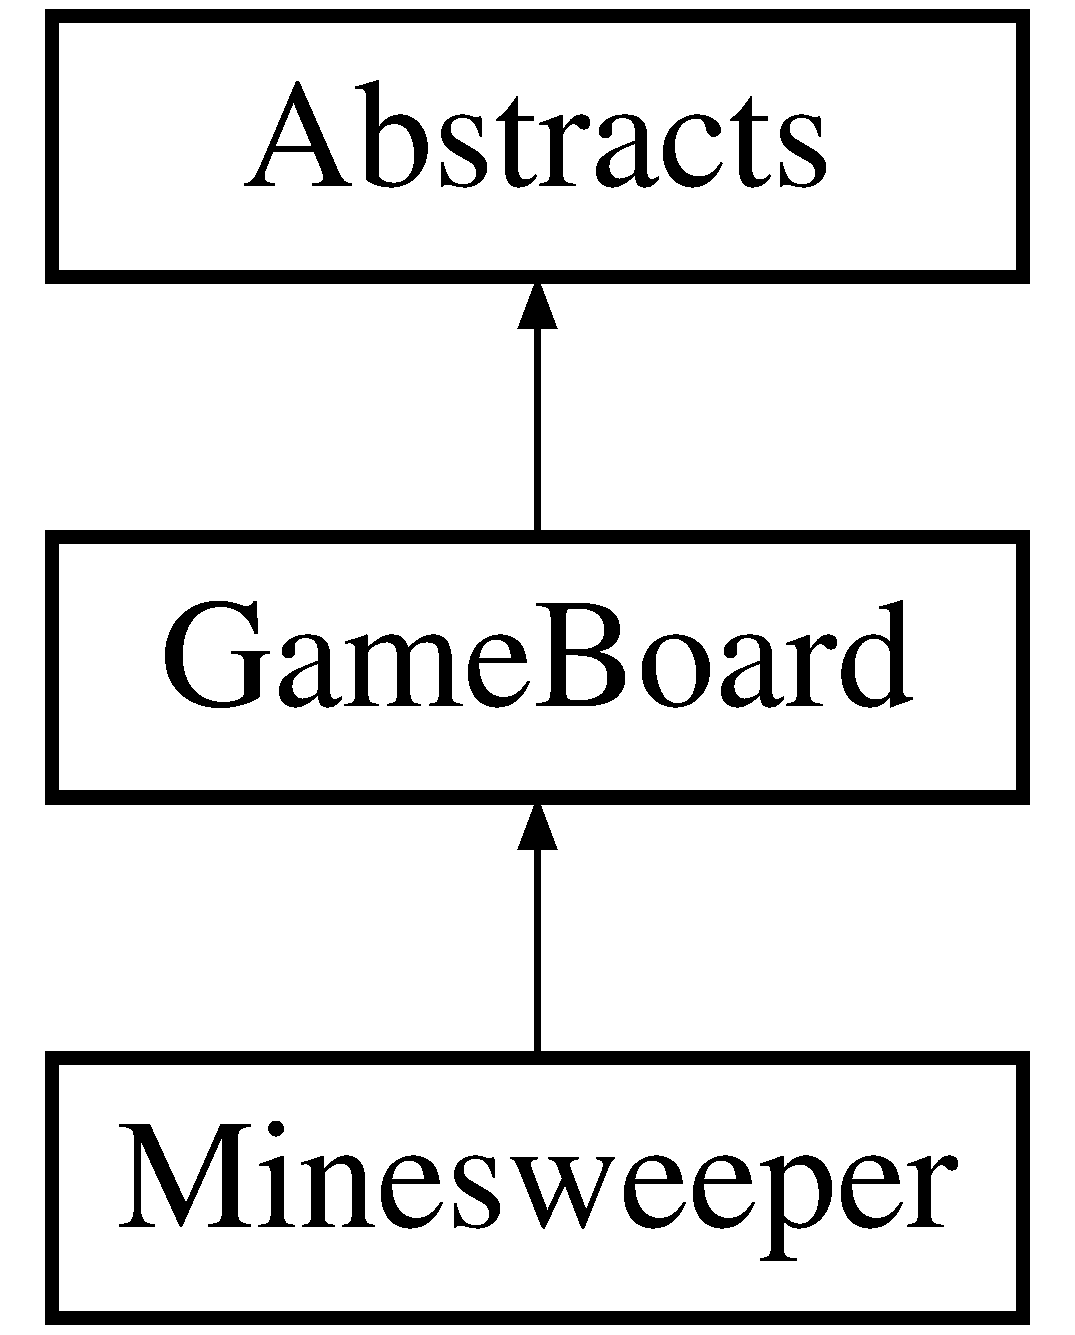
\includegraphics[height=3.000000cm]{class_minesweeper}
\end{center}
\end{figure}
\subsection*{Public Member Functions}
\begin{DoxyCompactItemize}
\item 
\hyperlink{class_minesweeper_a289ffbe6b9e6b728a19d1f73b78262e2}{Minesweeper} (int row, int col)
\item 
void \hyperlink{class_minesweeper_ab316cfe272f38e4768a6e45c171bce3a}{set\+Rows} (int)
\item 
void \hyperlink{class_minesweeper_a6e243fa0d9859fcf6dc4e45ec146b7df}{set\+Cols} (int)
\item 
int \hyperlink{class_minesweeper_abf6ccbfbecf96ef15f21ca7a94e98f1b}{get\+Rows} () const 
\item 
int \hyperlink{class_minesweeper_a82c571f6a7a80d001a3cb0a73445588f}{get\+Cols} () const 
\item 
void \hyperlink{class_minesweeper_ac158ba4f4bca146302059096db943dad}{print} () const 
\item 
void \hyperlink{class_minesweeper_ab90b8a53aee9758259e690bcb397bb1e}{prnt\+Obscr} () const 
\begin{DoxyCompactList}\small\item\em Function prints the \hyperlink{class_minesweeper}{Minesweeper} with spaces hidden. \end{DoxyCompactList}\item 
void \hyperlink{class_minesweeper_ac5ae43be99a0cc126da239d3572acbe7}{set\+Up\+G} ()
\item 
void \hyperlink{class_minesweeper_a98b38257079a4541fdb5ac8f1f9d25db}{play\+Game} ()
\item 
void \hyperlink{class_minesweeper_a9304b49877a6d02f6e5b9c5f48f34055}{clear} ()
\begin{DoxyCompactList}\small\item\em Function that clears the grid on which game will be played. \end{DoxyCompactList}\item 
void \hyperlink{class_minesweeper_ab8e0fb7bce67aa24dd2e616a2f37917d}{save\+Game} ()
\item 
void \hyperlink{class_minesweeper_aa7c5b407fa1907a07a29c9a04d23a3f2}{rules} ()
\item 
void \hyperlink{class_minesweeper_a11b4462ac060a000e79f5537b9ca9da2}{load\+Game} ()
\item 
int \hyperlink{class_minesweeper_ae83bf3ccb6d130ca8ef1ce642e1fc136}{get\+Mines} () const 
\item 
\hyperlink{class_minesweeper}{Minesweeper} \& \hyperlink{class_minesweeper_ad32e6a1ddc9ade6f3958c7568f994e9a}{operator=} (const \hyperlink{class_minesweeper}{Minesweeper} \&)
\end{DoxyCompactItemize}
\subsection*{Additional Inherited Members}


\subsection{Detailed Description}
This is the class that holds the \hyperlink{class_minesweeper}{Minesweeper} as well as the associated flags that occur when a user selects a square 

\subsection{Constructor \& Destructor Documentation}
\hypertarget{class_minesweeper_a289ffbe6b9e6b728a19d1f73b78262e2}{}\index{Minesweeper@{Minesweeper}!Minesweeper@{Minesweeper}}
\index{Minesweeper@{Minesweeper}!Minesweeper@{Minesweeper}}
\subsubsection[{Minesweeper(int row, int col)}]{\setlength{\rightskip}{0pt plus 5cm}Minesweeper\+::\+Minesweeper (
\begin{DoxyParamCaption}
\item[{int}]{row, }
\item[{int}]{col}
\end{DoxyParamCaption}
)\hspace{0.3cm}{\ttfamily [inline]}}\label{class_minesweeper_a289ffbe6b9e6b728a19d1f73b78262e2}


\subsection{Member Function Documentation}
\hypertarget{class_minesweeper_a9304b49877a6d02f6e5b9c5f48f34055}{}\index{Minesweeper@{Minesweeper}!clear@{clear}}
\index{clear@{clear}!Minesweeper@{Minesweeper}}
\subsubsection[{clear()}]{\setlength{\rightskip}{0pt plus 5cm}void Minesweeper\+::clear (
\begin{DoxyParamCaption}
{}
\end{DoxyParamCaption}
)\hspace{0.3cm}{\ttfamily [virtual]}}\label{class_minesweeper_a9304b49877a6d02f6e5b9c5f48f34055}


Function that clears the grid on which game will be played. 

Make sure each square is empty 

Reimplemented from \hyperlink{class_game_board_a85f26da7e1be97961225f8fd893f18ee}{Game\+Board}.

\hypertarget{class_minesweeper_a82c571f6a7a80d001a3cb0a73445588f}{}\index{Minesweeper@{Minesweeper}!get\+Cols@{get\+Cols}}
\index{get\+Cols@{get\+Cols}!Minesweeper@{Minesweeper}}
\subsubsection[{get\+Cols() const }]{\setlength{\rightskip}{0pt plus 5cm}int Minesweeper\+::get\+Cols (
\begin{DoxyParamCaption}
{}
\end{DoxyParamCaption}
) const\hspace{0.3cm}{\ttfamily [inline]}, {\ttfamily [virtual]}}\label{class_minesweeper_a82c571f6a7a80d001a3cb0a73445588f}


Reimplemented from \hyperlink{class_game_board_a3e72c802e556c00efd911d95986a4f2e}{Game\+Board}.

\hypertarget{class_minesweeper_ae83bf3ccb6d130ca8ef1ce642e1fc136}{}\index{Minesweeper@{Minesweeper}!get\+Mines@{get\+Mines}}
\index{get\+Mines@{get\+Mines}!Minesweeper@{Minesweeper}}
\subsubsection[{get\+Mines() const }]{\setlength{\rightskip}{0pt plus 5cm}int Minesweeper\+::get\+Mines (
\begin{DoxyParamCaption}
{}
\end{DoxyParamCaption}
) const\hspace{0.3cm}{\ttfamily [inline]}}\label{class_minesweeper_ae83bf3ccb6d130ca8ef1ce642e1fc136}
\hypertarget{class_minesweeper_abf6ccbfbecf96ef15f21ca7a94e98f1b}{}\index{Minesweeper@{Minesweeper}!get\+Rows@{get\+Rows}}
\index{get\+Rows@{get\+Rows}!Minesweeper@{Minesweeper}}
\subsubsection[{get\+Rows() const }]{\setlength{\rightskip}{0pt plus 5cm}int Minesweeper\+::get\+Rows (
\begin{DoxyParamCaption}
{}
\end{DoxyParamCaption}
) const\hspace{0.3cm}{\ttfamily [inline]}, {\ttfamily [virtual]}}\label{class_minesweeper_abf6ccbfbecf96ef15f21ca7a94e98f1b}


Reimplemented from \hyperlink{class_game_board_a06b193fdd5b618efdbb2700fd7dcffd0}{Game\+Board}.

\hypertarget{class_minesweeper_a11b4462ac060a000e79f5537b9ca9da2}{}\index{Minesweeper@{Minesweeper}!load\+Game@{load\+Game}}
\index{load\+Game@{load\+Game}!Minesweeper@{Minesweeper}}
\subsubsection[{load\+Game()}]{\setlength{\rightskip}{0pt plus 5cm}void Minesweeper\+::load\+Game (
\begin{DoxyParamCaption}
{}
\end{DoxyParamCaption}
)\hspace{0.3cm}{\ttfamily [virtual]}}\label{class_minesweeper_a11b4462ac060a000e79f5537b9ca9da2}
Function prints the data variable from the \hyperlink{class_minesweeper}{Minesweeper} structure writen to a binary file \hyperlink{class_minesweeper_ac158ba4f4bca146302059096db943dad}{print()}; 

Reimplemented from \hyperlink{class_game_board_ac73c2de2d5a31c591ff3434d8fd38686}{Game\+Board}.

\hypertarget{class_minesweeper_ad32e6a1ddc9ade6f3958c7568f994e9a}{}\index{Minesweeper@{Minesweeper}!operator=@{operator=}}
\index{operator=@{operator=}!Minesweeper@{Minesweeper}}
\subsubsection[{operator=(const Minesweeper \&)}]{\setlength{\rightskip}{0pt plus 5cm}{\bf Minesweeper} \& Minesweeper\+::operator= (
\begin{DoxyParamCaption}
\item[{const {\bf Minesweeper} \&}]{rhs}
\end{DoxyParamCaption}
)}\label{class_minesweeper_ad32e6a1ddc9ade6f3958c7568f994e9a}
\hypertarget{class_minesweeper_a98b38257079a4541fdb5ac8f1f9d25db}{}\index{Minesweeper@{Minesweeper}!play\+Game@{play\+Game}}
\index{play\+Game@{play\+Game}!Minesweeper@{Minesweeper}}
\subsubsection[{play\+Game()}]{\setlength{\rightskip}{0pt plus 5cm}void Minesweeper\+::play\+Game (
\begin{DoxyParamCaption}
{}
\end{DoxyParamCaption}
)}\label{class_minesweeper_a98b38257079a4541fdb5ac8f1f9d25db}
Play a game of minesweeper User inputs how many rows and columns and the difficulty Select the row

User wants to save the game save the game and exit

check bounds

Select the column

check bounds

end\+Time

Prepare to print completed \hyperlink{class_minesweeper}{Minesweeper}

Print the complete \hyperlink{class_minesweeper}{Minesweeper} \hypertarget{class_minesweeper_ac158ba4f4bca146302059096db943dad}{}\index{Minesweeper@{Minesweeper}!print@{print}}
\index{print@{print}!Minesweeper@{Minesweeper}}
\subsubsection[{print() const }]{\setlength{\rightskip}{0pt plus 5cm}void Minesweeper\+::print (
\begin{DoxyParamCaption}
{}
\end{DoxyParamCaption}
) const\hspace{0.3cm}{\ttfamily [virtual]}}\label{class_minesweeper_ac158ba4f4bca146302059096db943dad}
Functions prints the \hyperlink{class_minesweeper}{Minesweeper} with all the squares revealed. used mostly after player loses 

Reimplemented from \hyperlink{class_game_board_a90f93cc1b6ca4e06f7200696fb21c9b9}{Game\+Board}.

\hypertarget{class_minesweeper_ab90b8a53aee9758259e690bcb397bb1e}{}\index{Minesweeper@{Minesweeper}!prnt\+Obscr@{prnt\+Obscr}}
\index{prnt\+Obscr@{prnt\+Obscr}!Minesweeper@{Minesweeper}}
\subsubsection[{prnt\+Obscr() const }]{\setlength{\rightskip}{0pt plus 5cm}void Minesweeper\+::prnt\+Obscr (
\begin{DoxyParamCaption}
{}
\end{DoxyParamCaption}
) const}\label{class_minesweeper_ab90b8a53aee9758259e690bcb397bb1e}


Function prints the \hyperlink{class_minesweeper}{Minesweeper} with spaces hidden. 

Print the column index

Pad initial output of column indicator

K\+E\+E\+P E\+M\+P\+T\+Y spaces and M\+I\+N\+Es hidden

print out the C\+L\+E\+A\+Red area

Print out the actual value of the square \hypertarget{class_minesweeper_aa7c5b407fa1907a07a29c9a04d23a3f2}{}\index{Minesweeper@{Minesweeper}!rules@{rules}}
\index{rules@{rules}!Minesweeper@{Minesweeper}}
\subsubsection[{rules()}]{\setlength{\rightskip}{0pt plus 5cm}void Minesweeper\+::rules (
\begin{DoxyParamCaption}
{}
\end{DoxyParamCaption}
)}\label{class_minesweeper_aa7c5b407fa1907a07a29c9a04d23a3f2}
\hypertarget{class_minesweeper_ab8e0fb7bce67aa24dd2e616a2f37917d}{}\index{Minesweeper@{Minesweeper}!save\+Game@{save\+Game}}
\index{save\+Game@{save\+Game}!Minesweeper@{Minesweeper}}
\subsubsection[{save\+Game()}]{\setlength{\rightskip}{0pt plus 5cm}void Minesweeper\+::save\+Game (
\begin{DoxyParamCaption}
{}
\end{DoxyParamCaption}
)}\label{class_minesweeper_ab8e0fb7bce67aa24dd2e616a2f37917d}
\hypertarget{class_minesweeper_a6e243fa0d9859fcf6dc4e45ec146b7df}{}\index{Minesweeper@{Minesweeper}!set\+Cols@{set\+Cols}}
\index{set\+Cols@{set\+Cols}!Minesweeper@{Minesweeper}}
\subsubsection[{set\+Cols(int)}]{\setlength{\rightskip}{0pt plus 5cm}void Minesweeper\+::set\+Cols (
\begin{DoxyParamCaption}
\item[{int}]{col}
\end{DoxyParamCaption}
)\hspace{0.3cm}{\ttfamily [virtual]}}\label{class_minesweeper_a6e243fa0d9859fcf6dc4e45ec146b7df}


Reimplemented from \hyperlink{class_game_board_a84673c141f4790940df3aca0e24c3203}{Game\+Board}.

\hypertarget{class_minesweeper_ab316cfe272f38e4768a6e45c171bce3a}{}\index{Minesweeper@{Minesweeper}!set\+Rows@{set\+Rows}}
\index{set\+Rows@{set\+Rows}!Minesweeper@{Minesweeper}}
\subsubsection[{set\+Rows(int)}]{\setlength{\rightskip}{0pt plus 5cm}void Minesweeper\+::set\+Rows (
\begin{DoxyParamCaption}
\item[{int}]{row}
\end{DoxyParamCaption}
)\hspace{0.3cm}{\ttfamily [virtual]}}\label{class_minesweeper_ab316cfe272f38e4768a6e45c171bce3a}


Reimplemented from \hyperlink{class_game_board_ac8b28f17c3ea049f3cb07216b850c4a9}{Game\+Board}.

\hypertarget{class_minesweeper_ac5ae43be99a0cc126da239d3572acbe7}{}\index{Minesweeper@{Minesweeper}!set\+Up\+G@{set\+Up\+G}}
\index{set\+Up\+G@{set\+Up\+G}!Minesweeper@{Minesweeper}}
\subsubsection[{set\+Up\+G()}]{\setlength{\rightskip}{0pt plus 5cm}void Minesweeper\+::set\+Up\+G (
\begin{DoxyParamCaption}
{}
\end{DoxyParamCaption}
)\hspace{0.3cm}{\ttfamily [virtual]}}\label{class_minesweeper_ac5ae43be99a0cc126da239d3572acbe7}
Get the user name

ask user if they want to play

play if answer is yes

Get game information from user

Get new data only if user wants to continue

Information was invalid

Cleanup 

Reimplemented from \hyperlink{class_game_board_a81f25c1109558131e0153a4b278cffcb}{Game\+Board}.



The documentation for this class was generated from the following files\+:\begin{DoxyCompactItemize}
\item 
\hyperlink{_minesweeper_8h}{Minesweeper.\+h}\item 
\hyperlink{_minesweeper_8cpp}{Minesweeper.\+cpp}\end{DoxyCompactItemize}

\hypertarget{class_game_board_1_1wrong}{}\section{Game\+Board\+:\+:wrong Class Reference}
\label{class_game_board_1_1wrong}\index{Game\+Board\+::wrong@{Game\+Board\+::wrong}}


output this if user tries to set negative rows or columns  




{\ttfamily \#include $<$Game\+Board.\+h$>$}



\subsection{Detailed Description}
output this if user tries to set negative rows or columns 

The documentation for this class was generated from the following file\+:\begin{DoxyCompactItemize}
\item 
\hyperlink{_game_board_8h}{Game\+Board.\+h}\end{DoxyCompactItemize}

\chapter{File Documentation}
\hypertarget{_8dep_8inc}{}\section{.dep.\+inc File Reference}
\label{_8dep_8inc}\index{.\+dep.\+inc@{.\+dep.\+inc}}

\hypertarget{_abstracts_8h}{}\section{Abstracts.\+h File Reference}
\label{_abstracts_8h}\index{Abstracts.\+h@{Abstracts.\+h}}
\subsection*{Classes}
\begin{DoxyCompactItemize}
\item 
class \hyperlink{class_abstracts}{Abstracts}
\end{DoxyCompactItemize}

\hypertarget{_game_board_8cpp}{}\section{Game\+Board.\+cpp File Reference}
\label{_game_board_8cpp}\index{Game\+Board.\+cpp@{Game\+Board.\+cpp}}
{\ttfamily \#include $<$iostream$>$}\\*
{\ttfamily \#include \char`\"{}game\+Board.\+h\char`\"{}}\\*

\hypertarget{_game_board_8h}{}\section{Game\+Board.\+h File Reference}
\label{_game_board_8h}\index{Game\+Board.\+h@{Game\+Board.\+h}}
{\ttfamily \#include \char`\"{}Abstracts.\+h\char`\"{}}\\*
\subsection*{Classes}
\begin{DoxyCompactItemize}
\item 
class \hyperlink{class_game_board}{Game\+Board}
\begin{DoxyCompactList}\small\item\em Base class for games that require an n$\ast$m array such as minesweeper. \end{DoxyCompactList}\item 
class \hyperlink{class_game_board_1_1wrong}{Game\+Board\+::wrong}
\begin{DoxyCompactList}\small\item\em output this if user tries to set negative rows or columns \end{DoxyCompactList}\end{DoxyCompactItemize}

\hypertarget{main_8cpp}{}\section{main.\+cpp File Reference}
\label{main_8cpp}\index{main.\+cpp@{main.\+cpp}}
{\ttfamily \#include $<$iostream$>$}\\*
{\ttfamily \#include $<$cstdlib$>$}\\*
{\ttfamily \#include $<$ctime$>$}\\*
{\ttfamily \#include $<$vector$>$}\\*
{\ttfamily \#include $<$iomanip$>$}\\*
{\ttfamily \#include \char`\"{}Minesweeper.\+h\char`\"{}}\\*
{\ttfamily \#include \char`\"{}Templates.\+h\char`\"{}}\\*
\subsection*{Functions}
\begin{DoxyCompactItemize}
\item 
void \hyperlink{main_8cpp_aec22e45a418810f5b7df4cf6eb169e68}{Game\+Rules} ()
\item 
int \hyperlink{main_8cpp_ac0f2228420376f4db7e1274f2b41667c}{main} (int argc, const char $\ast$argv\mbox{[}$\,$\mbox{]})
\end{DoxyCompactItemize}


\subsection{Function Documentation}
\hypertarget{main_8cpp_aec22e45a418810f5b7df4cf6eb169e68}{}\index{main.\+cpp@{main.\+cpp}!Game\+Rules@{Game\+Rules}}
\index{Game\+Rules@{Game\+Rules}!main.\+cpp@{main.\+cpp}}
\subsubsection[{Game\+Rules()}]{\setlength{\rightskip}{0pt plus 5cm}void Game\+Rules (
\begin{DoxyParamCaption}
{}
\end{DoxyParamCaption}
)}\label{main_8cpp_aec22e45a418810f5b7df4cf6eb169e68}
\hypertarget{main_8cpp_ac0f2228420376f4db7e1274f2b41667c}{}\index{main.\+cpp@{main.\+cpp}!main@{main}}
\index{main@{main}!main.\+cpp@{main.\+cpp}}
\subsubsection[{main(int argc, const char $\ast$argv[])}]{\setlength{\rightskip}{0pt plus 5cm}int main (
\begin{DoxyParamCaption}
\item[{int}]{argc, }
\item[{const char $\ast$}]{argv\mbox{[}$\,$\mbox{]}}
\end{DoxyParamCaption}
)}\label{main_8cpp_ac0f2228420376f4db7e1274f2b41667c}
call function here to show the game rules

Cast for random time seed generator

error output

Exit stage right 
\hypertarget{_minesweeper_8cpp}{}\section{Minesweeper.\+cpp File Reference}
\label{_minesweeper_8cpp}\index{Minesweeper.\+cpp@{Minesweeper.\+cpp}}
{\ttfamily \#include $<$fstream$>$}\\*
{\ttfamily \#include $<$iostream$>$}\\*
{\ttfamily \#include $<$cstdlib$>$}\\*
{\ttfamily \#include $<$ctime$>$}\\*
{\ttfamily \#include $<$string$>$}\\*
{\ttfamily \#include $<$iomanip$>$}\\*
{\ttfamily \#include \char`\"{}Minesweeper.\+h\char`\"{}}\\*

\hypertarget{_minesweeper_8h}{}\section{Minesweeper.\+h File Reference}
\label{_minesweeper_8h}\index{Minesweeper.\+h@{Minesweeper.\+h}}
{\ttfamily \#include $<$string$>$}\\*
{\ttfamily \#include \char`\"{}Game\+Board.\+h\char`\"{}}\\*
\subsection*{Classes}
\begin{DoxyCompactItemize}
\item 
class \hyperlink{class_minesweeper}{Minesweeper}
\end{DoxyCompactItemize}

\hypertarget{_templates_8h}{}\section{Templates.\+h File Reference}
\label{_templates_8h}\index{Templates.\+h@{Templates.\+h}}
\subsection*{Classes}
\begin{DoxyCompactItemize}
\item 
class \hyperlink{class_game}{Game$<$ T $>$}
\end{DoxyCompactItemize}

%--- End generated contents ---

% Index
\backmatter
\newpage
\phantomsection
\clearemptydoublepage
\addcontentsline{toc}{chapter}{Index}
\printindex

\end{document}
